
%%%%%%%%%%%%%%%%%%%%%%%%%%%%%%%%%%%%%%%%%%%%%%%%%%%%%%%%%%%%%%%%%%%%%%%%%%%%%%%%%%%%%%%%%%%%%%%%%%%%%%%
%%%%%%%%%%%%%% Template de Artigo Adaptado para Trabalho de Diplomação do ICEI %%%%%%%%%%%%%%%%%%%%%%%%
%% codificação UTF-8 - Abntex - Latex -  							     %%
%% Autor:    Fábio Leandro Rodrigues Cordeiro  (fabioleandro@pucminas.br)                            %% 
%% Co-autor: Prof. João Paulo Domingos Silva  e Harison da Silva                                     %%
%% Revisores normas NBR (Padrão PUC Minas): Helenice Rego Cunha e Prof. Theldo Cruz                  %%
%% Versão: 1.0     13 de março 2014                                                                  %%
%%%%%%%%%%%%%%%%%%%%%%%%%%%%%%%%%%%%%%%%%%%%%%%%%%%%%%%%%%%%%%%%%%%%%%%%%%%%%%%%%%%%%%%%%%%%%%%%%%%%%%%
\section{\esp Introdução}
A princípio, achar em um grafo direcionado todas as rotas que não se cruzam em arestas, dados o vértice de raiz e o vértice de destino, parece algo trivial e sem muitas implicações plausíveis para problemas reais.

 Porém, após esse primeiro contato com assunto, vimos o quão importante é este problema pois, existem muitos problemas reais que podem ser modelados como caminhos disjuntos em arestas. Por exemplo, um sistema de suporte à decisão em gerenciamento de fluxo de tráfego aéreo, ou ainda, redes de roteamento de transmissão múltipla obtidas a partir de uma rede geral de comunicações.
 
Para acharmos uma solução para tal problema utilizaremos uma modelagem que inferi os grafos como ponderados, ou seja, todas as arestas terão peso 1 e iremos usar um dos algoritmos de fluxo da teoria de grafos, o Algoritmo de Edmonds-Karp para encontrar todos os caminhos disjuntos em arestas.



\section{\esp Metodologia}

A resolução do problema é dividida em dois arquivos, \textit{graph.cpp} que é responsável
pela representação e operações em grafos e \textit{main.cpp} que lida com as entradas e saídas.

O arquivo \textit{graphGenerator.cpp}\cite{sanfoundry} foi criado com o propósito de gerar grafos com proporções
maiores para testar os limites dos algoritmos implementados.

Em \textit{main.cpp}, é importado o arquivo \textit{graph.cpp}, que contém todas as bibliotecas 
padrão da linguagem C++ usadas no projeto. A monitorização do tempo de execução do programa
é realizada no arquivo \textit{main.cpp} e conta o tempo que o programa demorou para achar os 
caminhos disjuntos.

A classe graph, definida em \textit{graph.cpp}, possui 5 campos, um vetor 2D de inteiross, 
que representa a matrix de adjacência, um inteiro que representa o número de caminhos disjuntos
calculados antecipadamente, um inteiro que representa o número de caminhos disjuntos obtido pelo
algoritmo, um vetor de tuplas, que armazena os caminhos encontrados pelo algoritmo e por fim
há dois inteiros que guardam o valor do número de vértices e arestas respectivamente.

\newpage
Dentro os métodos da classe graph, se destacam graph\_from\_txt(), 
vector<int> obtain\_successors(int vertex, vector<vector<int>> graph) , 
bool breadth\_first\_search(vector<vector<int>> graph,int rootVertex, int targetVertex, vector<int> \&parents) e
void find\_unique\_paths(). O primeiro se responsabiliza por criar um grafo a partir do padrão de .txt
usado pelo grupo, que segue o padrão a seguir: \newline
n1 n2 n3\newline
v0 v1\newline
v0 v2\newline
...\newline
vn v(n1-1)\newline
\newline
n1 representa o número de vértices, n2 representa o número de arestas, n3 representa o número de 
caminhos disjuntos, em seguida, todas a n2 arestas são representadas pelo vértice de saída e de 
entrada.\newline
O segundo obtém os n vértices sucessores de um vértice vertex em um grafo graph, o terceiro 
realiza uma busca em largura em um grafo graph, do vértice rootVertex até o vértice targetVertex,
preenchendo o array parents com os pais de cada vértice e retorna se encontrou caminho entre os
vértices rootVertex e targetVertex. Por fim, o último encontra os caminhos disjuntos de um grafo,
tendo como grafo source o que se encontra na posição 0 e grafo terminal o que se encontra na última
posição. Ele faz isso colocando todas as arestas com peso 1 e obtendo o fluxo máximo desse grafo por meio
do método de Edmonds-Karp\cite{gfg}.Ao se obter o fluxo máximo, um grafo novo somente com as arestas que  possuem fluxo, eliminando todas as arestas não utilizadas pelo grafo, em seguida, os caminhos são extraídos desse grafo e são inseridos no vetor de caminhos da classe.




\section{\esp Resultados}

Nesta seção serão apresentados os resultados dos testes realizados usando nosso programa e os dados de 
teste criados automaticamente e manualmente.


\begin{comment}


\begin{enumerate}



\subsection{\esp Grafos Utilizados}

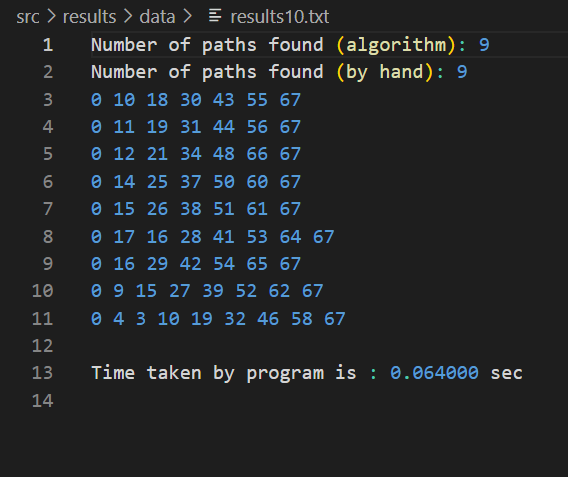
\includegraphics[scale=0.5]{figuras/R10.png}


\end{enumerate}


\end{comment}

\subsection{\esp Algoritmo para se encontrar número máximo de caminhos disjuntos }
O algoritmo implementado (complexidade $O(n^4)$ ou $O(EV^3)$) resolve esse problema de forma ótima.
Ele realiza a busca em largura (complexidade $O(n^2)$ ou $O(V^2)$ dado ao uso de matriz de adjacência)
no máximo $O(n^2)$ $O(EV)$ vezes.

\begin{enumerate}

    \item O primeiro grafo conta com 15 vértices e 29 arestas:
    \begin{center}
        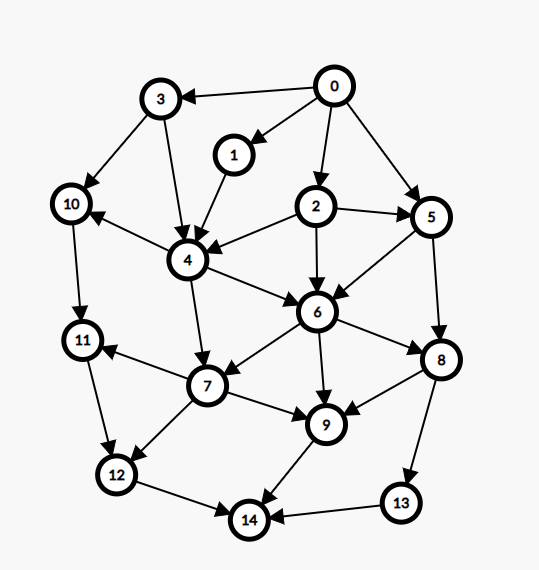
\includegraphics[scale=0.35]{figuras/Grafo1.png}
    \end{center}
    Solução ótima: 3 caminhos\newline
    Solução encontrada pelo algoritmo: 3 caminhos\newline
    Caminhos encontrados pelo algoritmo:\newline
    0 5 6 9 14 \newline
    0 1 4 7 12 14 \newline
    0 2 4 6 8 13 14 \newline

    \item O segundo grafo conta com 15 vértices e 21 arestas:
    \begin{center}
        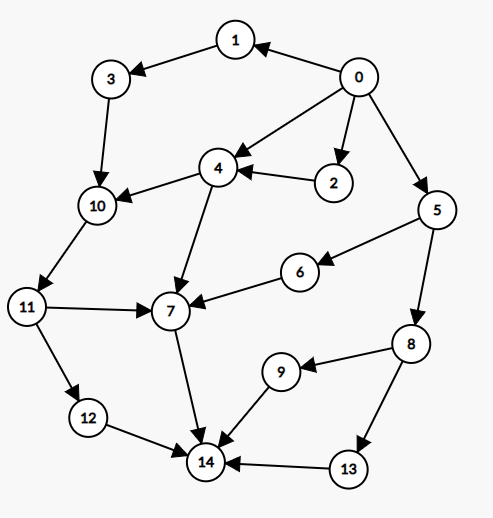
\includegraphics[scale=0.5]{figuras/Grafo2.png}
    \end{center}
    Solução ótima: 3 caminhos\newline
    Solução encontrada pelo algoritmo: 3 caminhos\newline
    Caminhos encontrados pelo algoritmo:\newline
    0 5 8 9 14 \newline
    0 4 7 14 \newline
    0 1 3 10 11 12 14 \newline
    
    
    \item O terceiro grafo conta com 18 vértices e 37 arestas:
    \begin{center}
        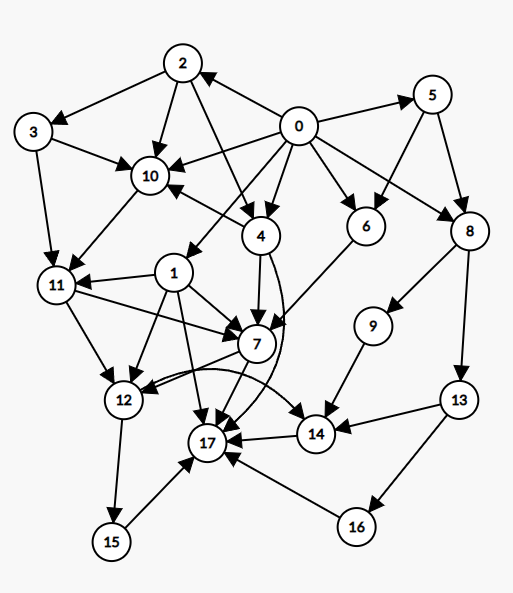
\includegraphics[scale=0.4]{figuras/Grafo3.png}
    \end{center}
    Solução ótima: 6 caminhos\newline
    Solução encontrada pelo algoritmo: 6 caminhos\newline
    Caminhos encontrados pelo algoritmo:\newline
    0 10 11 7 17 \newline
    0 6 14 17 \newline
    0 1 17 \newline
    0 4 17 \newline
    0 8 13 16 17 \newline
    0 5 6 7 12 15 17 \newline
    
    \item O quarto grafo conta com 23 vértices e 36 arestas:
    \begin{center}
        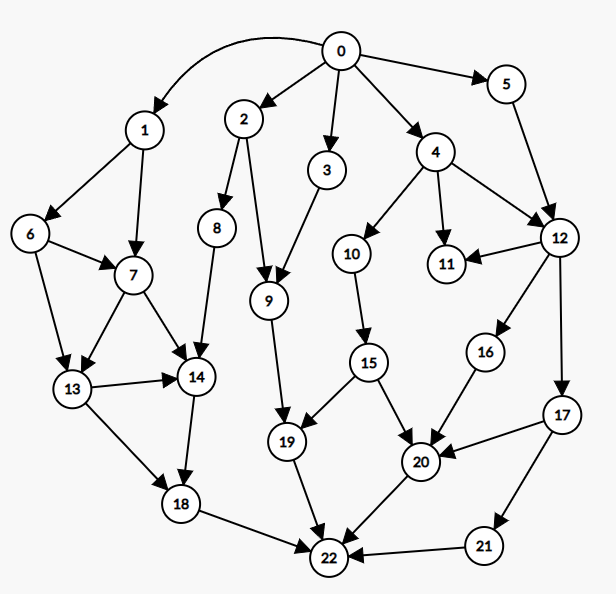
\includegraphics[scale=0.4]{figuras/Grafo4.png}
    \end{center}
    Solução ótima: 4 caminhos\newline
    Solução encontrada pelo algoritmo: 4 caminhos\newline
    Caminhos encontrados pelo algoritmo:\newline
    0 4 10 15 20 22 \newline
    0 5 12 17 21 22 \newline
    0 2 9 19 22 \newline
    0 1 6 13 18 22 \newline
    
    \item O quinto grafo conta com 23 vértices e 44 arestas:
    \begin{center}
        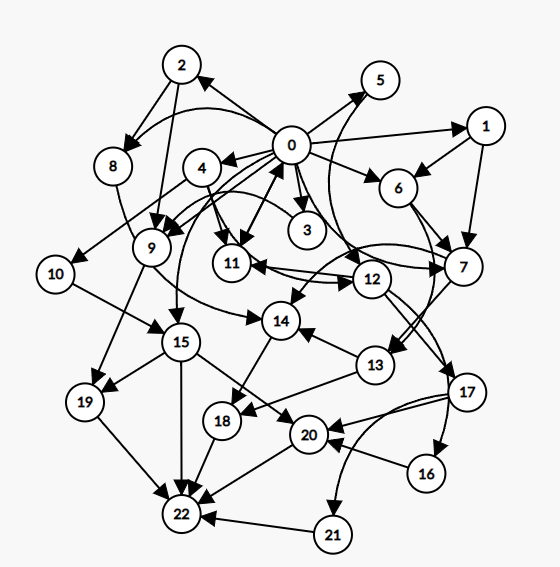
\includegraphics[scale=0.4]{figuras/Grafo5.png}
    \end{center}
    Solução ótima: 5 caminhos\newline
    Solução encontrada pelo algoritmo: 5 caminhos\newline
    Caminhos encontrados pelo algoritmo:\newline
    0 15 22 \newline
    0 9 19 22 \newline
    0 6 13 18 22 \newline
    0 4 10 15 20 22 \newline
    0 5 12 17 21 22 \newline
    
    \item O sexto grafo conta com 16 vértices e 27 arestas:
    \begin{center} 
        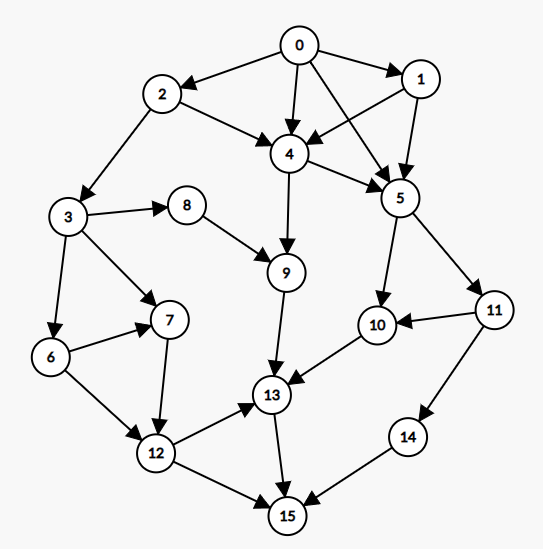
\includegraphics[scale=0.5]{figuras/Grafo6.png}
    \end{center}
    Solução ótima: 3 caminhos\newline
    Solução encontrada pelo algoritmo: 3 caminhos\newline
    Caminhos encontrados pelo algoritmo:\newline
    0 4 9 13 15 \newline
    0 5 11 14 15 \newline
    0 2 3 6 12 15 \newline

    
    \item O setimo grafo conta com 16 vértices e 18 arestas:
    \begin{center}
        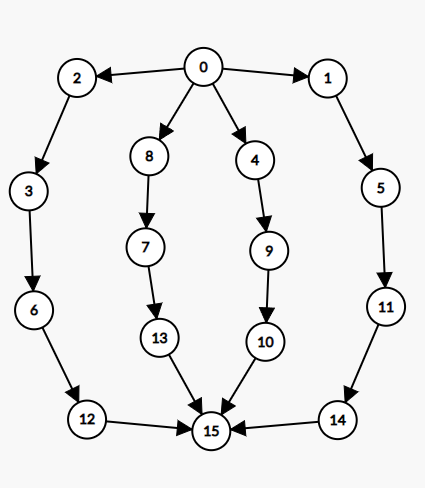
\includegraphics[scale=0.5]{figuras/Grafo7.png}
    \end{center}
    Solução ótima: 4 caminhos\newline
    Solução encontrada pelo algoritmo: 4 caminhos\newline
    Caminhos encontrados pelo algoritmo:\newline
    0 4 9 10 15 \newline
    0 8 7 13 15 \newline
    0 1 5 11 14 15 \newline
    0 2 3 6 12 15 \newline

    
    \item O oitavo grafo conta com 16 vértices e 23 arestas:
    \begin{center}
        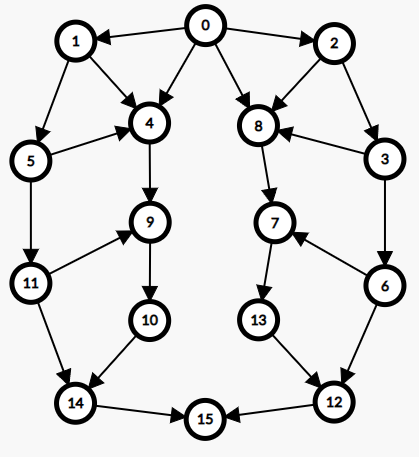
\includegraphics[scale=0.4]{figuras/Grafo8.png}
    \end{center}
    Solução ótima: 2 caminhos\newline
    Solução encontrada pelo algoritmo: 2 caminhos\newline
    Caminhos encontrados pelo algoritmo:\newline
    0 1 5 11 14 15 \newline
    0 2 3 6 12 15 \newline
    
    \item O nono grafo conta com 16 vértices e 28 arestas:
    \begin{center}
        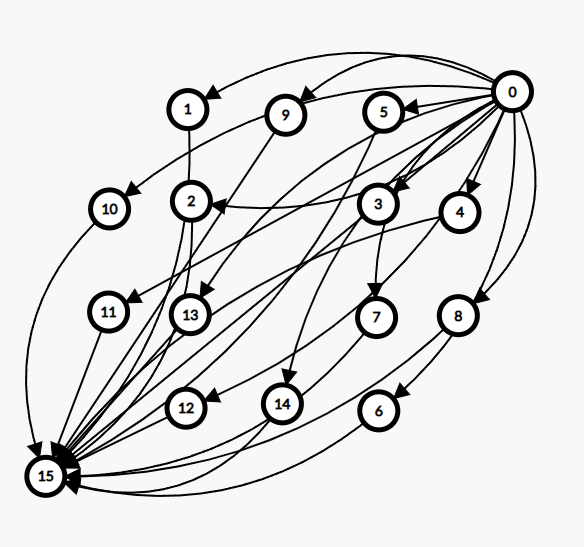
\includegraphics[scale=0.5]{figuras/Grafo9.png}
    \end{center}
    Solução ótima: 15 caminhos\newline
    Solução encontrada pelo algoritmo: 15 caminhos\newline
    Caminhos encontrados pelo algoritmo:\newline
    0 1 15 \newline
    0 2 15 \newline
    0 3 15 \newline
    0 4 15 \newline
    0 5 15 \newline
    0 6 15 \newline
    0 7 15 \newline
    0 8 15 \newline
    0 9 15 \newline
    0 10 15 \newline
    0 11 15 \newline
    0 12 15 \newline
    0 13 15 \newline
    0 14 15 \newline
    
    \item O decimo grafo conta com 68 vértices e 118 arestas:
    \begin{center}  
        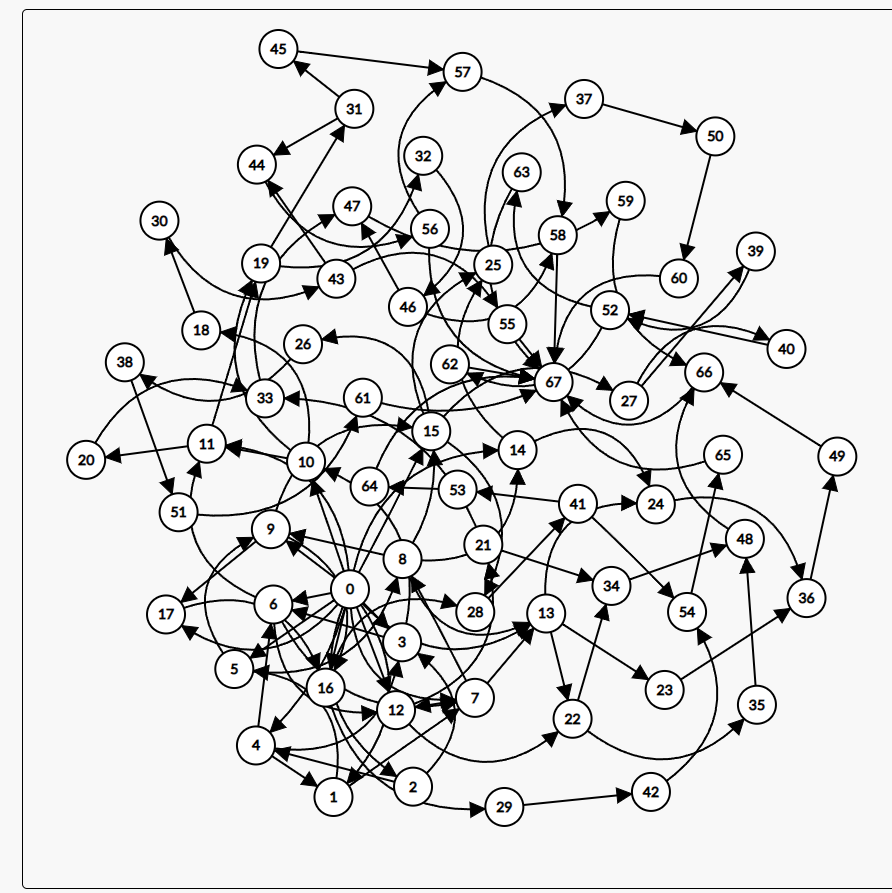
\includegraphics[scale=0.3]{figuras/G10.png}
    \end{center}
    Solução ótima: 9 caminhos\newline
    Solução encontrada pelo algoritmo: 9 caminhos\newline
    Caminhos encontrados pelo algoritmo:\newline
    0 10 18 30 43 55 67 \newline
    0 11 19 31 44 56 67 \newline
    0 12 21 34 48 66 67 \newline
    0 14 25 37 50 60 67 \newline
    0 15 26 38 51 61 67 \newline
    0 17 16 28 41 53 64 67 \newline
    0 16 29 42 54 65 67 \newline
    0 9 15 27 39 52 62 67 \newline
    0 4 3 10 19 32 46 58 67 \newline

\end{enumerate}

\subsection{\esp Análise de vértices por tempo em grafos}
 Os grafos criados automaticamente nos permitem testar os limites do algoritmo implementado. Foram
 gerados grafos de $2^n$ vértices e $4*2^n$ arestas para um n de 4 à 14. Isso é um intervalo de 16
 a 8192 vértices e 64 a 32768 arestas.

 
 
 
\begin{tikzpicture}
    \begin{axis}[
        xmin = 0, xmax = 8500,
        ymin = 0, ymax = 6500,
        grid = both,    
        width = 0.75\textwidth,
        height = 0.5\textwidth,
        xlabel = {Vértices},
        ylabel = {Tempo em segundos},
        ]
\addplot[
    smooth,
    thin,
    black,
] file[skip first] {vertTime.dat};
        \end{axis}
\end{tikzpicture}




\section{\esp Conclusão}

A partir dos resultados obtidos nos testes, podemos concluir que o método proposto é viável, uma vez 
que o tempo de execução é polinomial e a sua solução é ótima. Além disso, seu tempo de execução
não segue $O(n^4)$ para os grafos testados, seguindo um crescimento linear nos grafos de teste.